% 问题三由正文移入的补充检验；数值来源和版本见 support_materials/q3_validation_notes.md。
\section{问题三的补充检验}\label{sec:q3_appendix}
\renewcommand{\thesubsection}{\Alph{section}.\arabic{subsection}}

本附录保留展望长度、分源残差修正及旧方案诊断的详细记录，用于说明模型改进依据。历史实验沿用当时的初值设置，不能与正文从 $2$ 月 $1$ 日 $6000$ kWh 出发的正式结果直接混合比较。正式修正参数由一月标定确定，历史全年网格不用于重新选择参数。

\subsection{展望长度与分源残差修正的历史对照}

历史基准为 $24$ h 展望加 $\beta\sigma$ 光伏缓冲，其中 $\sigma$ 表示历史光伏残差的标准差，$\beta$ 为缓冲系数。表~\ref{tab:q3_ablation} 保留不同展望长度和修正方式的结果；分源残差修正启用后不再叠加该缓冲。

\begin{table}[!htbp]
  \centering
  \small
  \setlength{\tabcolsep}{4.5pt}
  \caption{历史展望长度与分源残差修正对照（沿用各历史实验初值）}
  \label{tab:q3_ablation}
  \begin{tabular}{lrrrr}
    \toprule
    变体 & 全年总费用/元 & 相对基线/元 & 紧急电量/kWh & 日末贴底天数 \\
    \midrule
    $24$h $+\beta$（基线） & 13{,}458{,}730.30 & 0 & 82{,}228.36 & 106 \\
    $48$h $+\beta$ & 13{,}421{,}219.84 & $-37{,}510.46$ & 70{,}433.46 & 0 \\
    $24$h $+q_L{=}0.65$ & 13{,}294{,}093.95 & $-164{,}636.35$ & 44{,}783.43 & 37 \\
    $48$h $+q_L{=}0.60$ & 13{,}274{,}667.54 & $-184{,}062.76$ & 58{,}355.20 & 1 \\
    $48$h $+q_L{=}0.65$ & 13{,}263{,}910.99 & $-194{,}819.31$ & 39{,}678.65 & 1 \\
    \bottomrule
  \end{tabular}
\end{table}

由表~\ref{tab:q3_ablation} 可见，历史记录中延长展望和采用分源残差修正均对应较低费用，前者还减少了日末储电量贴近下限的天数。这些对照支持将次日需求和预测误差纳入购电决策；鉴于历史初值设置的差异，表内费用差额不作为严格控制其他条件后的单因素贡献。

全年历史网格在 $q_L=0.65$ 时费用较低，正式方案仍按一月标定取 $q_L=0.60$。同一历史回放口径下，$48$ h 展望取 $q_L=0.60,0.65,0.70$ 的总费用分别为 $13{,}274{,}667.54$、$13{,}263{,}910.99$、$13{,}308{,}698.92$ 元，说明所选参数附近费用变化较小；完整历史网格见支撑材料 \texttt{q3\_validation\_notes.md}。

\subsection{旧方案的紧急购电诊断}

旧 $24$ h 加 $\beta\sigma$ 方案全年紧急购电为 $82{,}228.36$ kWh，其中 $88.8\%$ 与储能电量耗尽相关，$20{:}00$--$21{:}00$ 占紧急电量的 $47.4\%$，日末贴近储能下限的天数为 $106$ 天。其逐小时构成见图~\ref{fig:q3_failure}。

\begin{figure}[!htbp]
  \centering
  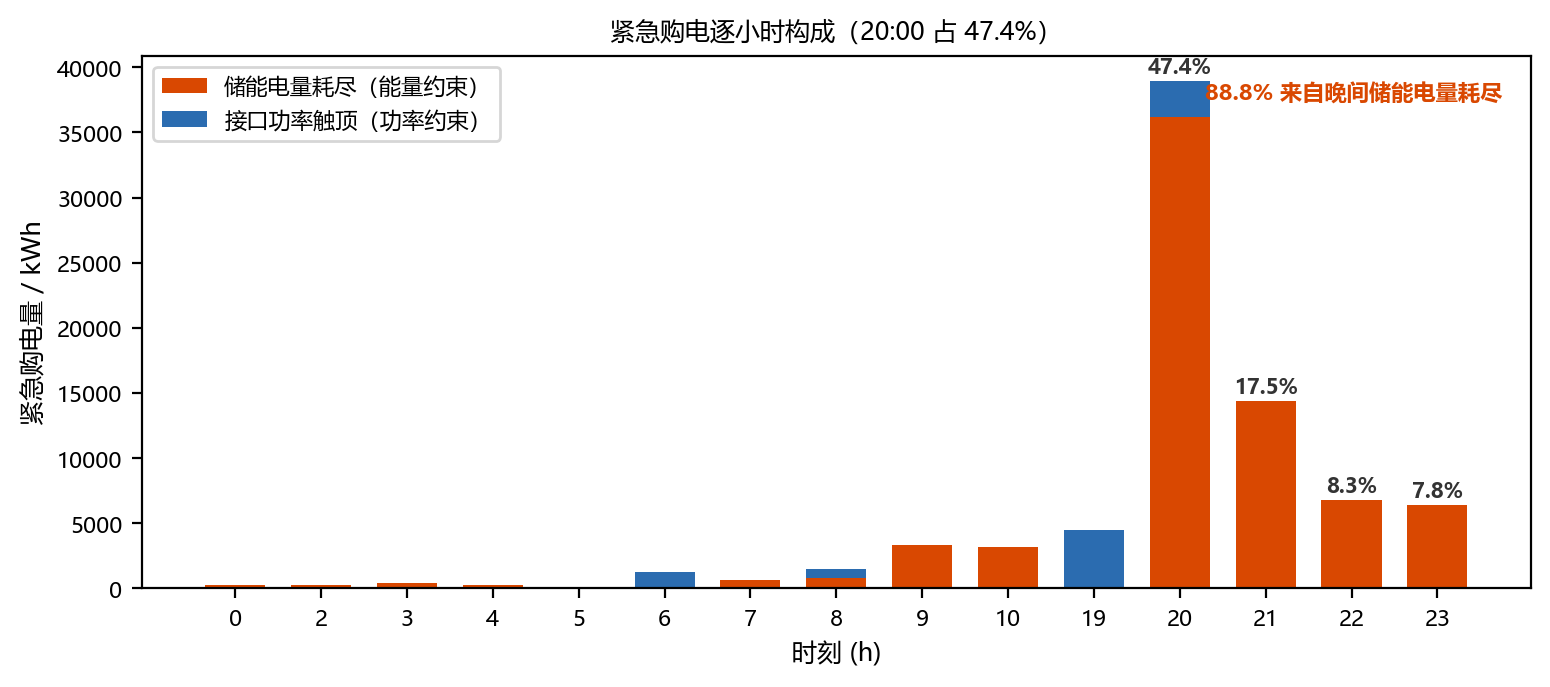
\includegraphics[width=0.82\linewidth]{fig_q3_emergency.png}
  \caption{旧方案（$24$h $+\beta\sigma$）全年紧急购电的逐小时构成：$88.8\%$ 来自电量耗尽
  （SOC 触底）而非接口功率触顶，$20{:}00$ 单小时占 $47.4\%$}
  \label{fig:q3_failure}
\end{figure}

由图~\ref{fig:q3_failure} 可见，旧方案的紧急购电主要集中在晚间储能电量耗尽时段，因此需要在签订购电合同阶段考虑晚间及跨日电量需求。上述比例属于旧方案；正式 LA 的日末贴底天数为 $1$ 天，不能将旧方案的诊断比例当作正式方案的统计结果。

\subsection{短期完美信息对照与初值敏感性}

在 $2$ 月 $1$--$14$ 日窗口内，以当天真实负荷和光伏作为已知输入进行单日优化，得到完美信息对照费用 $585{,}705.84$ 元；同期 LA 为 $636{,}942.33$ 元，N0 为 $653{,}094.43$ 元。LA 比该对照高约 $8.7\%$，同时低于不调整方案。该结果仅用于短期比较，不能据此将全部费用差距归因于预测误差，也不替代全年同口径策略对照。

历史 LA 以一月末约 $8377$ kWh 为二月初值，全年费用为 $13{,}274{,}667.54$ 元。正式回放从 $6000$ kWh 出发，总费用为 $13{,}275{,}795.85$ 元，增加约 $1128$ 元，占正式费用的 $0.0085\%$。该对照下初值变化对全年费用影响较小，正文统一采用后者。
